\bookmark[page=1,level=0]{Page de garde}

\begin{titlepage}
  \newgeometry{top=1cm,bottom=1cm,left=1cm,right=1cm}

	\begin{figure}
    \begin{center}
      \subfloat{
        
\includegraphics[width=5cm]{figures/garde/fig_logoUL.pdf}
      }
      \hfill
      \subfloat{
        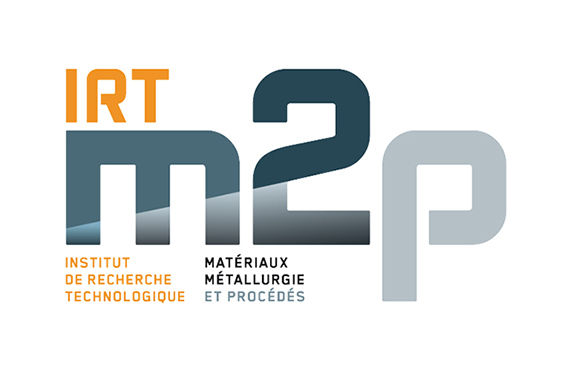
\includegraphics[width=5cm]{figures/garde/fig_logoIRT.jpeg}
      }
      \hfill
      \subfloat{
        
\includegraphics[width=5cm]{figures/garde/fig_logoIJL.png}
      }
    \end{center}
  \end{figure}

  \begin{center}
    \noindent
    \begin{minipage}{0.9\textwidth}\centering
  
    	\begin{center}
    		\setstretch{1.5}
    		
    		{\large THÈSE}\\
    		\vspace{5mm}
    
    		{\large Pour l'obtention du titre de}\\
        \vspace{5mm}
        		
    		{\bfseries\large DOCTEUR DE L'UNIVERSITÉ DE LORRAINE}\\
        {Science des Matériaux}
    		\vspace{5mm}
    		
    		{\normalsize présentée par}\\
    		\vspace{6mm}
    		
    		{\bfseries\large Walter Dal'Maz Silva}\\
    		\vspace{6mm}
  		
        {\rule{\textwidth}{2pt}\\
          \centering\Large\bfseries
          Mise au point de la carbonitruration gazeuse des alliages\\
          16NiCrMo13 et 23MnCrMo5: modélisation et procédés\\
          \rule{\textwidth}{2pt}
        }   
    	\end{center}
    		
    	\begin{flushleft}
    		\vspace{3mm} 
    		{\large Livré le {\today}.}
    	\end{flushleft}
    		
    	\vspace{2cm}
		
    	\begin{center}
    		\begin{tabbing}
    				\= Thierry BELMONTEEEEE
    				\= Ingénieur de Rechercheee, IJL, Nancyxx
    				\= Co-directeur de Th\kill\\
    				\>Jacky DULCY \>Ingénieur de Recherche, IJL, Nancy
    				\>Co-directeur de Thèse\\[5pt]
    				\>Thierry BELMONTE \>Directeur de Recherche, IJL, Nancy
    				\>Directeur de Thèse\\[5pt]
    		\end{tabbing}
    	\end{center}
    	\vfill
  	\end{minipage}
  \end{center}  	
\end{titlepage}
\newgeometry{tmargin=2.5cm,bmargin=2.5cm,lmargin=2.5cm,rmargin=2.5cm}
\newpage\thispagestyle{empty}\cleardoublepage
\endinput

%		{\large Institut Jean Lamour}\\
%		\vspace{5mm}
%		
%		{\large Institut de Recherche Technologique: Matériaux, Métallurgie et 
%		Procédés}\\
%		\vspace{5mm}
%		
%		{\large École Doctorale : Énergie Mécanique et Matériaux}\\
%		\vspace{6mm}